\subsubsection{微信小程序连接物联网}

随着安卓平台逐渐没落,多端开发应运而生,此时以Javascript、WXML布局的小程序便可以多端联合开发,而不用担心兼容性问题。
在此,我使用微信开发者工具 Stable 1.06.2407120 进行微信小程序开发,通过远程连接OneNET平台,随时随地,实时显示数据于手机当中。

\subsubsection{构建小程序UI}

基于Nodejs、Javascript语言,使用flex弹性布局,可以使得框架的构建更为简单。
此处的UI图标均采用互联网免费公开资料。

\begin{lstlisting} [language=HTML, caption=微信小程序UI]
    <!-- Title Header -->
    <view class = "container">
        <view class = "head_box">
            <image src = "/images/OneNET.jpg" mode =""/>
        <view>{{title}}</view>
          </view>
    <!-- Weather Module -->
          <view class = "weather_box">
            <view class = "welcome_text">
                  {{welcome}}
            </view>
              <view class = "flex">
                  <view class = "width50">
                    <image src="/images/Weather.jpg" style="width: 200rpx; margin-top: 30rpx; margin-left: 30rpx;" mode="widthFix"/>
                  </view>
                  <view>
                    <view class= "location_text">
                        <image src="/images/located.jpg" style ="width: 20rpx; margin-top: 10rpx;" mode="widthFix"/><text
                        style="font-size: 24rpx;">{{location}}</text>
                    </view>
                    <view>
                        <view class = "temperature_text">
                            {{temperature}}°C
                        </view>
                    </view>
                  </view>
              </view>
          </view>
    <!-- Device Module -->
\end{lstlisting}

再根据实际需要配置实现情况index.wxss, index,js文件,初步实现框架如下所示:

\begin{figure} [H]
    \centering
    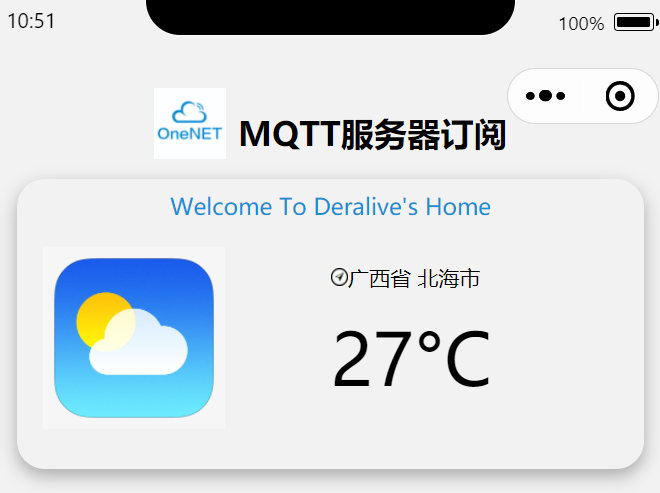
\includegraphics[width=0.3\textwidth]{img/WechatUI.png}
    \caption{微信小程序UI}
    \label{fig:WechatUI}
\end{figure}

根据OneNET平台提供的API,我们需要使用HTTP的GET请求连接到OneNET服务器,这里没办法使用Websocket协议(2024-02更新),

\begin{figure} [H]
    \centering
    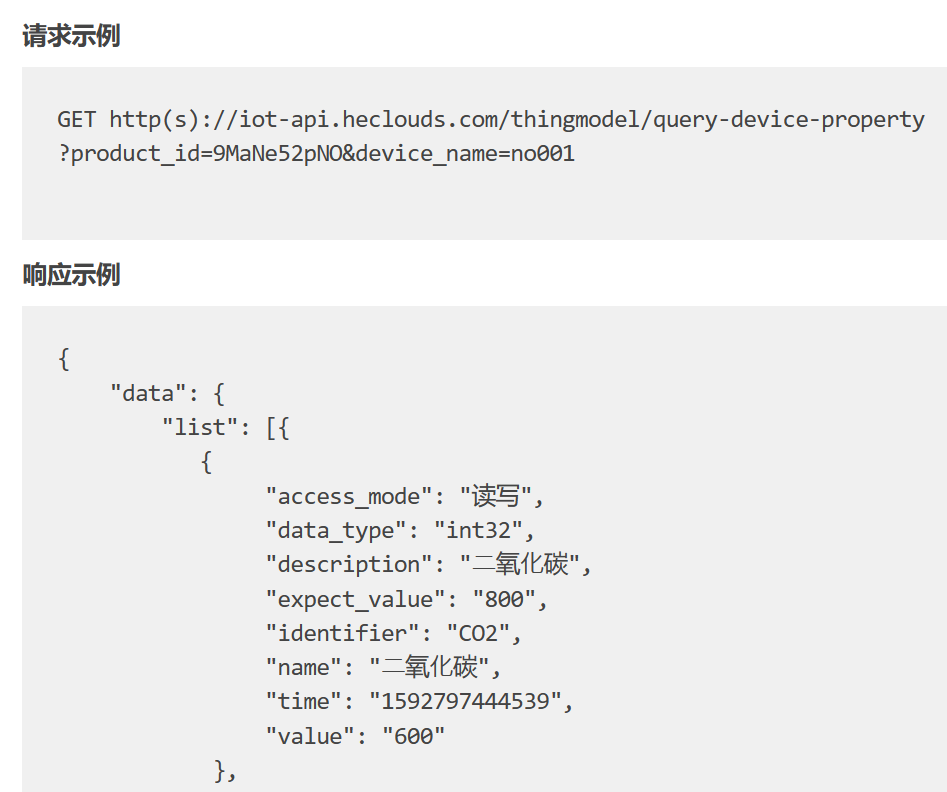
\includegraphics[width=0.35\textwidth]{img/GetMQTTDataHTTPGetExample.png}
    \caption{OneNET GET 请求示例}
    \label{fig:HTTP GET Example}
\end{figure}

按照示例模板,使用API-KEY,根据之前生成的鉴权参数(见图9),生成签名,并将其加入到请求头中,即可完成HTTP请求。

\begin{lstlisting} [language=C++, caption=HTTP GET 请求示例]
    getInfo() {
		let that = this;
		wx.request({
			url: "https://iot-api.heclouds.com/thingmodel/query-device-property?product_id=W9TI0JaXlu&device_name=DHT22",
			header: {
				"authorization": "version=2018-10-31&res=products%2FW9TI0JaXlu%2Fdevices%2FDHT22&et=1759306118&method=md5&sign=JRsZv0peZQOTmr7Eg8lGJg%3D%3D"
			},
			method: "GET",
			success: res => {
				console.log("获取成功", res);
            },
		});
	  },
\end{lstlisting}

获取JSON数据格式如下所示:

\begin{figure} [H]
    \centering
    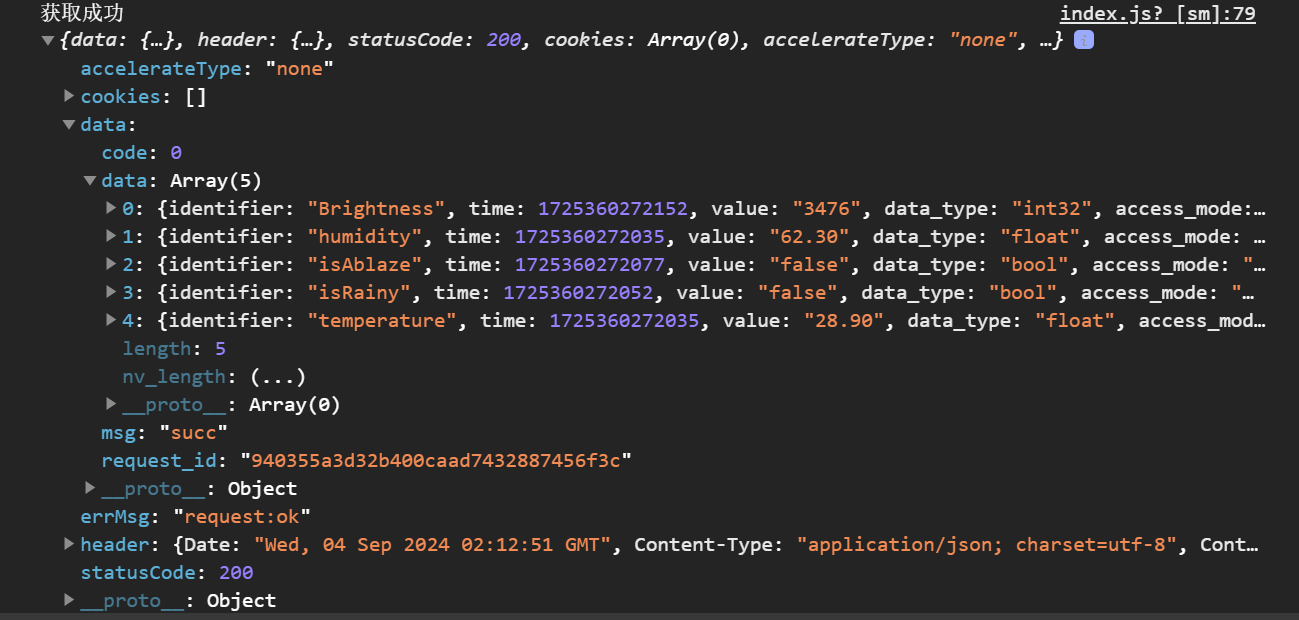
\includegraphics[width=0.45\textwidth]{img/GetMQTTJSON.png}
    \caption{OneNET JSON 数据格式}
    \label{fig:GetMQTTJSON}
\end{figure}

根据data.Array中的参数,每个数组返回的值代表不同的参数,后续只需读取逻辑即可。

\begin{lstlisting} [language=C++, caption=读取JSON数据]
    const sensorList = that.data.sensorList;
    sensorList[0].value = res.data.data[4].value;
    sensorList[1].value = res.data.data[1].value;
    sensorList[2].value = res.data.data[0].value;
    this.setData({
        sensorList: sensorList
    });
\end{lstlisting}

再使用WXML布局,将数据显示在UI上,即可完成微信小程序的连接物联网功能。

\begin{lstlisting} [language=HTML, caption=WXML布局]
    <!-- Sensor UI -->
	<view class = "sensors-system-title">
		传感器设备信息
	</view>
	<view class = "sensors-system">
		<view wx:for="{{sensorList}}" class = "system-info">
			<view class = "sensors-system-box1">
				<image src="{{item.img}}" style = "height: 80rpx; "mode="heightFix"/>
			</view>
			<view class = "sensors-system-box2">
				<view>{{item.parameter}}</view>
				<view>{{item.value}}{{item.unit}}</view>
				<view>{{item.name}}</view>
			</view>
		</view>
	</view>
</view>
\end{lstlisting}

\begin{figure} [H]
    \centering
    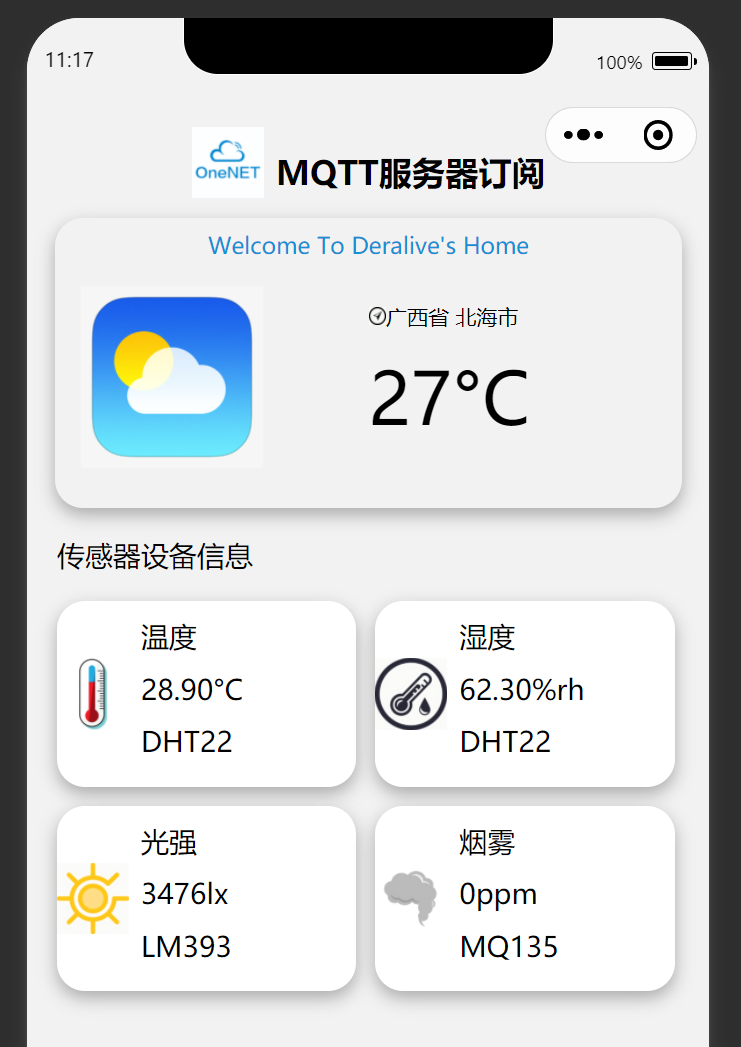
\includegraphics[width=0.2\textwidth]{img/FullUI.png}
    \caption{微信小程序完整UI}
    \label{fig:WechatUI2}
\end{figure}